现在有很多开源的数据集。考虑到本文要使用一些传统方法进行识别,我们选择的数据集不宜太大。
最终我们选择了kaggle上的Multilabel car and color dataset\footnote{可以在网站https://www.kaggle.com/datasets/julichitai/multilabel-small-car-and-color-dataset中获取。}作为数据集。
在数据集中,共包含三个品牌各三种颜色的车辆图片数据。数据集的部分图片如下:

\begin{figure}[H]
    \centering
\subfigure[matiz blue]{
    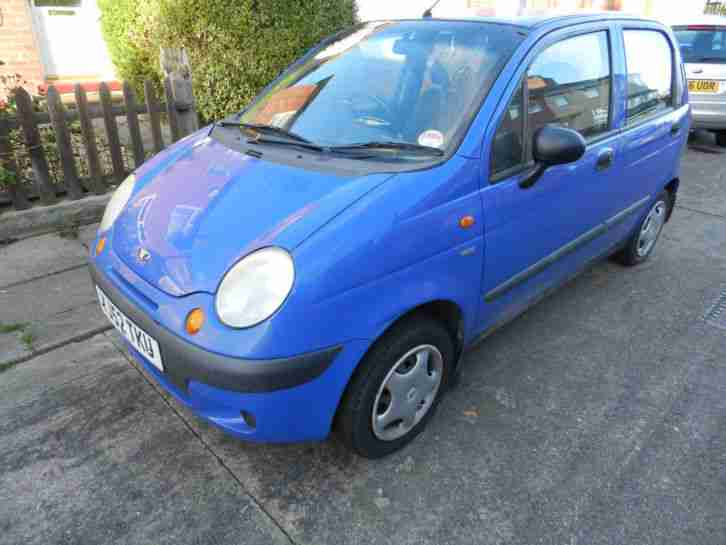
\includegraphics[width=3cm]{../dataset_graph/dataset_1.jpg}
    \label{matiz blue}
}\quad
\subfigure[tiggo black]{
    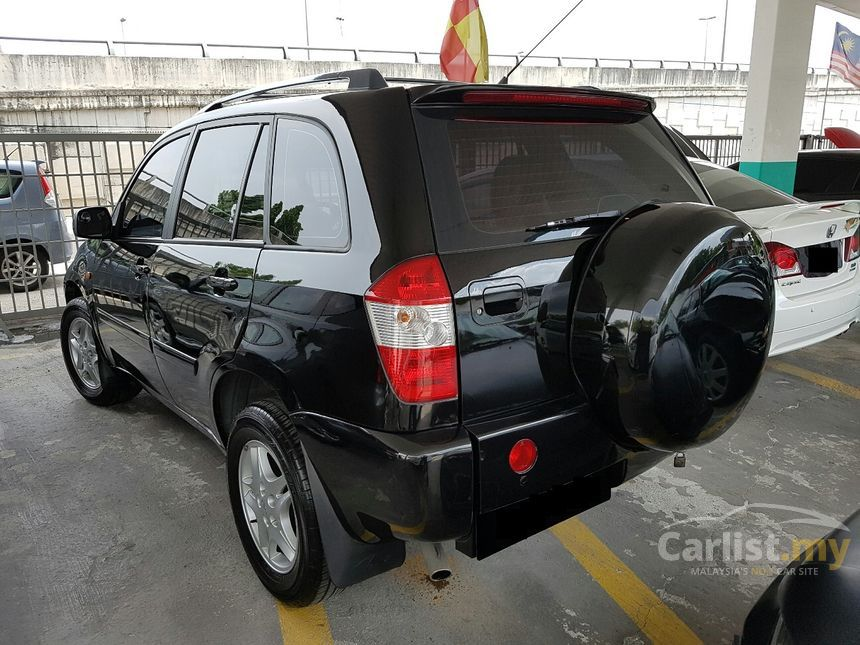
\includegraphics[width=3cm]{../dataset_graph/dataset_2.jpg}
        \label{tiggo black}
}\quad
\subfigure[rio blue]{
    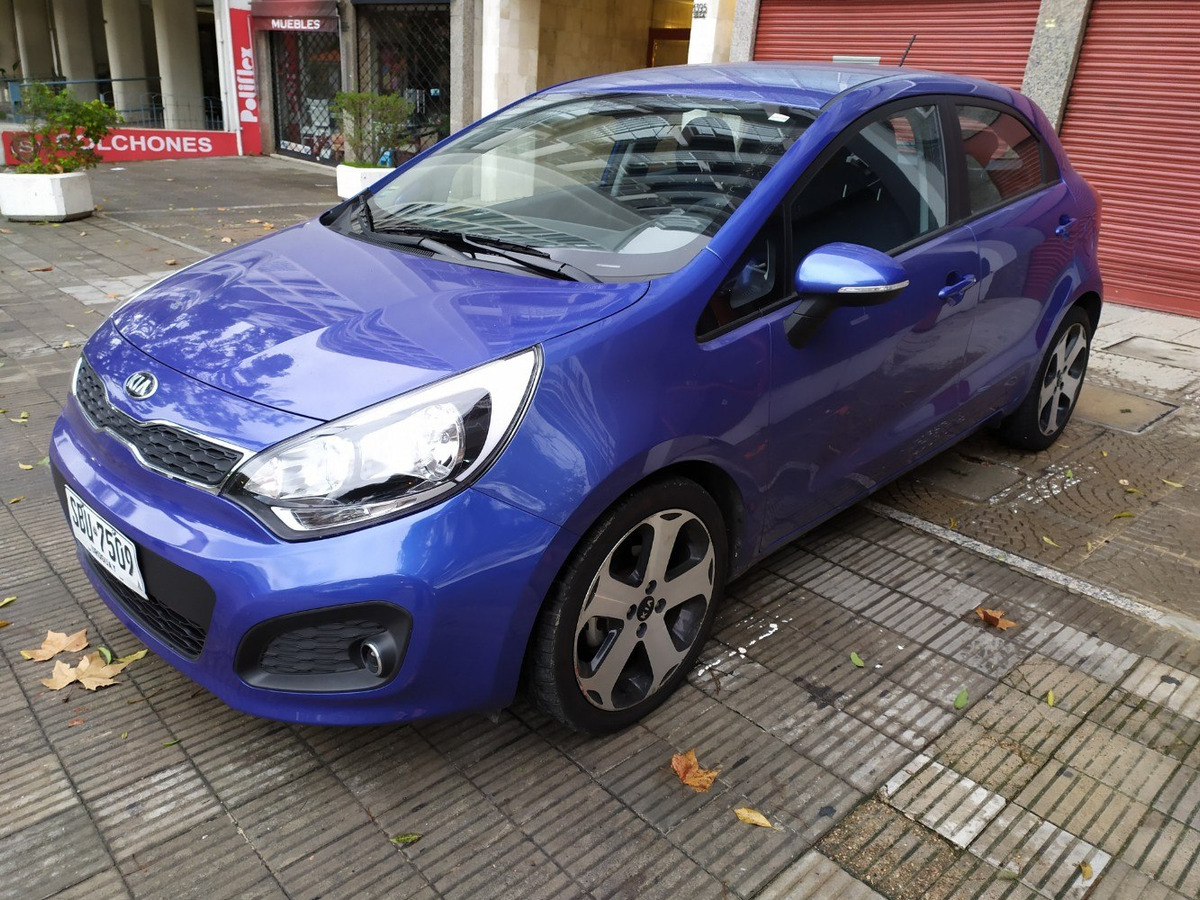
\includegraphics[width=3cm]{../dataset_graph/dataset_3.jpg}
    \label{rio blue}
}\quad
\subfigure[matiz red]{
    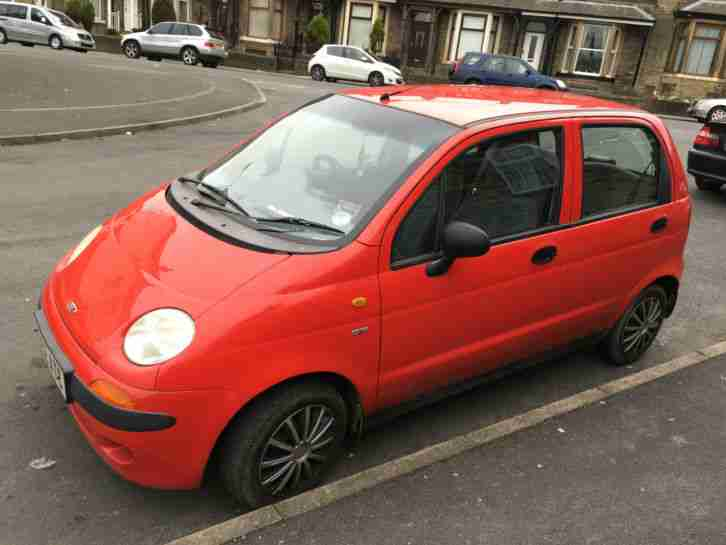
\includegraphics[width=3cm]{../dataset_graph/dataset_4.jpg}
    \label{matiz red}
}\quad
 
\caption{数据集样例}
\label{数据集样例}
\end{figure}

此数据集共有9个类,同时样本数量较少,不同品牌间视觉特征可能相近,如何提升模型泛化能力和防过拟合是关键。
此数据集很适合用来考察传统模型和神经网络之间的差别。